\documentclass[floatsintext,man]{apa6}

\usepackage{amssymb,amsmath}
\usepackage{ifxetex,ifluatex}
\usepackage{fixltx2e} % provides \textsubscript
\ifnum 0\ifxetex 1\fi\ifluatex 1\fi=0 % if pdftex
  \usepackage[T1]{fontenc}
  \usepackage[utf8]{inputenc}
\else % if luatex or xelatex
  \ifxetex
    \usepackage{mathspec}
    \usepackage{xltxtra,xunicode}
  \else
    \usepackage{fontspec}
  \fi
  \defaultfontfeatures{Mapping=tex-text,Scale=MatchLowercase}
  \newcommand{\euro}{€}
\fi
% use upquote if available, for straight quotes in verbatim environments
\IfFileExists{upquote.sty}{\usepackage{upquote}}{}
% use microtype if available
\IfFileExists{microtype.sty}{\usepackage{microtype}}{}

% Table formatting
\usepackage{longtable, booktabs}
\usepackage{lscape}
% \usepackage[counterclockwise]{rotating}   % Landscape page setup for large tables
\usepackage{multirow}		% Table styling
\usepackage{tabularx}		% Control Column width
\usepackage[flushleft]{threeparttable}	% Allows for three part tables with a specified notes section
\usepackage{threeparttablex}            % Lets threeparttable work with longtable

% Create new environments so endfloat can handle them
% \newenvironment{ltable}
%   {\begin{landscape}\begin{center}\begin{threeparttable}}
%   {\end{threeparttable}\end{center}\end{landscape}}

\newenvironment{lltable}
  {\begin{landscape}\begin{center}\begin{ThreePartTable}}
  {\end{ThreePartTable}\end{center}\end{landscape}}




% The following enables adjusting longtable caption width to table width
% Solution found at http://golatex.de/longtable-mit-caption-so-breit-wie-die-tabelle-t15767.html
\makeatletter
\newcommand\LastLTentrywidth{1em}
\newlength\longtablewidth
\setlength{\longtablewidth}{1in}
\newcommand\getlongtablewidth{%
 \begingroup
  \ifcsname LT@\roman{LT@tables}\endcsname
  \global\longtablewidth=0pt
  \renewcommand\LT@entry[2]{\global\advance\longtablewidth by ##2\relax\gdef\LastLTentrywidth{##2}}%
  \@nameuse{LT@\roman{LT@tables}}%
  \fi
\endgroup}


  \usepackage{graphicx}
  \makeatletter
  \def\maxwidth{\ifdim\Gin@nat@width>\linewidth\linewidth\else\Gin@nat@width\fi}
  \def\maxheight{\ifdim\Gin@nat@height>\textheight\textheight\else\Gin@nat@height\fi}
  \makeatother
  % Scale images if necessary, so that they will not overflow the page
  % margins by default, and it is still possible to overwrite the defaults
  % using explicit options in \includegraphics[width, height, ...]{}
  \setkeys{Gin}{width=\maxwidth,height=\maxheight,keepaspectratio}
\ifxetex
  \usepackage[setpagesize=false, % page size defined by xetex
              unicode=false, % unicode breaks when used with xetex
              xetex]{hyperref}
\else
  \usepackage[unicode=true]{hyperref}
\fi
\hypersetup{breaklinks=true,
            pdfauthor={},
            pdftitle={Child language experience in a Tseltal Mayan village},
            colorlinks=true,
            citecolor=blue,
            urlcolor=blue,
            linkcolor=black,
            pdfborder={0 0 0}}
\urlstyle{same}  % don't use monospace font for urls

\setlength{\parindent}{0pt}
%\setlength{\parskip}{0pt plus 0pt minus 0pt}

\setlength{\emergencystretch}{3em}  % prevent overfull lines


% Manuscript styling
\captionsetup{font=singlespacing,justification=justified}
\usepackage{csquotes}
\usepackage{upgreek}

 % Line numbering
  \usepackage{lineno}
  \linenumbers


\usepackage{tikz} % Variable definition to generate author note

% fix for \tightlist problem in pandoc 1.14
\providecommand{\tightlist}{%
  \setlength{\itemsep}{0pt}\setlength{\parskip}{0pt}}

% Essential manuscript parts
  \title{Child language experience in a Tseltal Mayan village}

  \shorttitle{Child language experience in a Tseltal Mayan village}


  \author{Marisa Casillas\textsuperscript{1}, Penelope Brown\textsuperscript{1}, \& Stephen C. Levinson\textsuperscript{1}}

  % \def\affdep{{"", "", ""}}%
  % \def\affcity{{"", "", ""}}%

  \affiliation{
    \vspace{0.5cm}
          \textsuperscript{1} Max Planck Institute for Psycholinguistics  }

  \authornote{
    Correspondence concerning this article should be addressed to Marisa
    Casillas, P.O. Box 310, 6500 AH Nijmegen, The Netherlands. E-mail:
    \href{mailto:Marisa.Casillas@mpi.nl}{\nolinkurl{Marisa.Casillas@mpi.nl}}
  }


  \abstract{We analyzed 9--11-hour at-home audio recordings from 10 Tseltal Mayan
children between 0;2 and 3;0 to investigate how often they engaged in
verbal interaction with others and whether their speech environment
changed with age, time of day, household size, and number of speakers
present. We found that Tseltal children are not often directly spoken
to, that most directed speech comes from adults, and that directed
speech does not increase with age. Most of children's directed speech
came in the mornings or early evenings, particularly for younger
children, and high interactional peaks tended to occur in
\textasciitilde{}1-minute bursts of turn taking. These findings only
partly support previous characterizations of Mayan caregiver-child talk.
An initial analysis of children's vocal development suggests that,
despite relatively little directed speech, these children develop early
language skills on a similar timescale to American English-learning
children. Given the present findings, we discuss multiple proposals for
how Tseltal children might be efficient learners.}
  \keywords{Child-directed speech, linguistic input, non-WEIRD, vocal maturity, turn
taking, interaction, Mayan \\

    \indent Word count: X
  }





\usepackage{amsthm}
\newtheorem{theorem}{Theorem}[section]
\newtheorem{lemma}{Lemma}[section]
\theoremstyle{definition}
\newtheorem{definition}{Definition}[section]
\newtheorem{corollary}{Corollary}[section]
\newtheorem{proposition}{Proposition}[section]
\theoremstyle{definition}
\newtheorem{example}{Example}[section]
\theoremstyle{definition}
\newtheorem{exercise}{Exercise}[section]
\theoremstyle{remark}
\newtheorem*{remark}{Remark}
\newtheorem*{solution}{Solution}
\begin{document}

\maketitle

\setcounter{secnumdepth}{0}



\section{Introduction}\label{intro}

A great deal of work in developmental language science revolves around
one central question: what linguistic evidence is needed to support
first language acquisition? In pursuing this topic, many researchers
have fixed their sights on the quantity and characteristics of speech
addressed to children (e.g., Golinkoff, Can, Soderstrom, \& Hirsh-Pasek,
2015; Hoff, 2006). In several languages, child-directed speech
(CDS\footnote{Throughout this article, we use \enquote{child-directed
  speech} and \enquote{CDS} in the most literal sense: speech designed
  for and directed toward a child recipient.}) has been demonstrated to
be distinct from adult-directed speech (ADS) in that it is
linguistically adapted for young listeners (Cristia, 2013; Soderstrom,
2007), interactionally rich (Bruner, 1983; Butterworth, 2003), preferred
by infants (Cooper \& Aslin, 1990; ManyBabies Collaborative, 2017; Segal
\& Newman, 2015), and appears to facilitate early word learning
(Cartmill et al., 2013; Hoff, 2003; Hurtado, Marchman, \& Fernald, 2008;
Rowe, 2008; Weisleder \& Fernald, 2013). However, ethnographic reports
from a number of traditional, non-Western communities suggest that
children easily acquire their language(s) even when they are only
infrequently directly addressed (Brown, 2011). If so, frequent CDS may
not be essential for learning language; just useful for facilitating
certain aspects of language development. In this paper we investigate
the language environment and early vocal development of 10 Tseltal Mayan
children growing up in a community where caregivers have previously been
reported to infrequently directly address speech to young children
(Brown, 1998b, 2011, 2014).

\subsection{Child-directed speech}\label{intro-cds}

Prior work in Western contexts has shown that the amount of CDS children
hear influences their language development; more CDS is associated with
faster-growing receptive and productive vocabularies (e.g., Hart \&
Risley, 1995; Hoff, 2003; Ramírez-Esparza, García-Sierra, \& Kuhl, 2014;
Shneidman \& Goldin-Meadow, 2012), faster lexical retrieval (Hurtado et
al., 2008; Weisleder \& Fernald, 2013), and faster syntactic development
(Huttenlocher, Waterfall, Vasilyeva, Vevea, \& Hedges, 2010). Given that
CDS is designed for a child hearer, it is more likely than ADS or
other-directed speech to align with the child's attention, and may
thereby comparatively facilitate early language development. There are,
however, a few significant caveats to this body of work relating CDS
quantity and language development.

First, while there is overwhelming evidence linking CDS quantity to
vocabulary size, links to grammatical development are more scant (but
see Brinchmann, Braeken, \& Lyster, 2019; Frank, Braginsky, Marchman, \&
Yurovsky, in preparation; Huttenlocher et al., 2010). While the
advantage of CDS for referential word learning is clear, it is less
obvious how it facilitates syntactic learning (see also Yurovsky, 2018).
On the other hand, there is a wealth of evidence that syntactic
knowledge is lexically specified (e.g., Goldberg, 2003; Lieven, Pine, \&
Baldwin, 1997), and that, crosslinguistically, children's vocabulary
size is one of the most robust predictors of their early syntactic
development (Bates \& Goodman, 1997; Frank et al., in preparation;
Marchman, Martínez-Sussmann, \& Dale, 2004)---what is good for the
lexicon may also be good for syntax. For now, a direct link between CDS
and grammatical development still needs further exploration .

Second, most work on CDS quantity uses summary measures that average
over the ebb and flow of the day (e.g., average proportion CDS). In
reality, verbal behaviors are highly structured during interaction:
while some occur at regular intervals , others occur in shorter, more
intense bursts separated by long periods of inactivity . Infants' and
adults' vocal behavior is clustered across multiple time scales of
daylong recordings (Abney, Smith, \& Yu, 2017) and noun and verb use is
bursty across languages (Blasi, Schikowski, Moran, Pfeiler, \& Stoll, in
preparation). Even in experimental settings, two-year-olds have been
shown to learn novel words better from a massed presentation of object
labels versus a distributed one (Schwab \& Lew-Williams, 2016; but see
Ambridge, Theakston, Lieven, \& Tomasello, 2006). The existence of
multi-scale temporal structure in children's language experience implies
new roles for attention and memory in development; more work is needed
to know how CDS is distributed over children's daily experiences
(Soderstrom \& Wittebolle, 2013).

Finally, prior work has typically focused on Western (primarily North
American) populations, limiting our ability to generalize effects of CDS
quantity (Brown \& Gaskins, 2014; Henrich, Heine, \& Norenzayan, 2010;
Lieven, 1994; M. Nielsen, Haun, Kärtner, \& Legare, 2017). While we gain
valuable insight by looking at within-population variation (e.g.,
different socioeconomic groups), we can more effectively find places
where our assumptions break down by studying new populations. Linguistic
anthropologists working in non-Western communities have long reported
that caregiver interaction styles vary immensely from place to place,
with some caregivers using little child-directed speech (Brown \&
Gaskins, 2014; Gaskins, 2006; Lieven, 1994; Ochs \& Schieffelin, 1984).
Children in these communities reportedly acquire language with
\enquote{typical}-looking benchmarks. For example, they start pointing
and talking around the same time we would expect for Western
middle-class infants (Brown, 2011, 2014; Brown \& Gaskins, 2014;
Liszkowski, Brown, Callaghan, Takada, \& De Vos, 2012; but see Salomo \&
Liszkowski, 2013). These findings have had little impact on mainstream
theories of language development, partly due to a lack of directly
comparable methods (Brown, 2014; Brown \& Gaskins, 2014). If, however,
children in these communities do acquire language without delay, despite
infrequent CDS, developmental language science would need to re-work
current ideas about the precise role of CDS quantity in early language
development.

Developmental language research using modern psycholinguistic methods
has supported the idea that children in some indigenous, non-Western
communities hear very little CDS. Scaff, Cristia, and colleagues (2017;
in preparation) estimate based on daylong recordings that Tsimane
children, growing up in a forager-horticulturalist population in the
Bolivian lowlands, hear maximally \textasciitilde{}4.8 minutes of CDS
per hour between 0;6 and 3;0 (Cristia et al., 2017; Scaff et al., in
preparation; see also Mastin \& Vogt, 2016; Vogt, Mastin, \& Schots,
2015).

Shneidman and colleagues (2010; 2012) analyzed speech from one-hour
at-home video recordings of children between 1;0 and 3;0 in a Yucatec
Mayan and a North American community. Their analyses yielded four main
findings: compared to the American children, (a) Yucatec children heard
many fewer utterances per hour, (b) a much smaller proportion of the
utterances they heard were child-directed, (c) the proportion of
utterances that were child-directed increased dramatically with age,
matching U.S. children's CDS proportion by 3;0, and (d) most of the
added CDS came from other children (e.g., older siblings/cousins). The
lexical diversity of the CDS Yucatec Mayan children heard at 24
months---particularly from adult speakers---predicted their vocabulary
knowledge at 35 months, suggesting that CDS characteristics still played
a role in that non-Western indigenous context.

\subsection{The current study}\label{intro-currentstudy}

We examine the early language experience of 10 Tseltal Mayan children
under age 3;0. Prior ethnographic work suggests that Tseltal caregivers
do not frequently use CDS until the children themselves begin to
actively initiate verbal interactions (Brown, 2011, 2014). Nonetheless,
Tseltal children develop language with no apparent delays (Brown, 2011,
2014; Brown \& Gaskins, 2014; Liszkowski et al., 2012).\footnote{For a
  review of comparative work on language socialization in Mayan cultures
  see Pye (2017).} We provide more details on the community and dataset
in the \protect\hyperlink{methods}{Methods section}. We analyze five
basic measures of Tseltal children's language environments including:
(a) the quantity of speech directed to them, (b) the quantity of
other-directed speech they could potentially overhear, (c) the rate of
contingent responses to their vocalizations, (d) the rate of their
contingent responses to others' vocalizations, and (e) the duration of
their interactional dyadic sequences. We then also roughly estimate the
number of minutes per day children spent in \enquote{high turn-taking}
interaction and outline a basic trajectory for their early vocal
development.

Based on prior work, we predicted that Tseltal Mayan children would be
infrequently directly addressed, that the amount of CDS and contingent
responses they heard would increase with age, that most CDS would come
from other children, and that, despite this, their early vocal
development would be on par with Western children. We additionally
predicted that children's language environments would be bursty---that
high-intensity interactions would be brief and sparsely distributed
throughout the day, accounting for the majority of children's daily CDS.

\hypertarget{methods}{\section{Methods}\label{methods}}

\subsection{Corpus}\label{methods-dataset}

The children in this dataset come from a small-scale, subsistence
farming community in the highlands of Chiapas (Southern Mexico). The
vast majority of children grow up speaking Tseltal monolingually at
home. Nuclear families are typically organized into patrlinieal clusters
of large, multi-generation households. More than forty years of
ethnographic work by the second author has supported the idea that
Tseltal children's language environments are non-child-centered and
non-object-centered (Brown, 1998b, 2011, 2014). During their waking
hours, infants are typically tied to their mother's back while she goes
about her work for the day. When not on their mother's back, young
children are often cared for by other family members, especially older
siblings. Typically, CDS is limited until children themselves begin to
initiate interactions, usually around age 1;0. Interactional exchanges,
when they do occur, are often brief or non-verbal (e.g., object exchange
routines) and take place within a multi-participant context (Brown,
2014). Interactions tend to focus on appropriate actions and responses
(not on words and their meanings), and young children are socialized to
attend the events taking place around them (see also de León, 2000,
2011; Rogoff, Paradise, Arauz, Correa-Chávez, \& Angelillo, 2003). By
age five, most children are competent speakers who engage in daily
chores and the caregiving of their younger siblings. The Tseltal
approach to caregiving is similar to that described for other Mayan
communities (de León, 2011; Gaskins, 1996, 1999; e.g., León, 1998; Pye,
1986; Rogoff et al., 1993, 2003; Shneidman \& Goldin-Meadow, 2012).

The current data come from the Casillas HomeBank Corpus (Casillas,
Brown, \& Levinson, 2017a; VanDam et al., 2016), which includes daylong
recordings and other developmental language data from more than 100
children under 4;0 across two indigenous, non-Western communities: the
Tseltal Mayan community described here and a Papua New Guinean community
described elsewhere (Brown, 2011, 2014; Brown \& Casillas, in press).
This Tseltal corpus, primarily collected in 2015, includes recordings
from 55 children born to 43 mothers. The participating families
typically only had 2--3 children (median = 2; range = 1--9), due to the
fact that they come from a young subsample of the community (mothers:
mean = 26.3 years; median = 25; range = 16--43 and fathers: mean = 30;
median = 27; range = 17---52). On average, mothers were 20 years old
when they had their first child (median = 19; range = 12--27), with a
following inter-child interval of 3 years (median = 2.8; range =
1--8.5).\footnote{These estimates do not include miscarriages or
  children who passed away.} As a result, 28\% of the participating
families had two children under 4;0. To our knowledge at time of
recording, all children were typically developing. Note that all ages
should be taken with a grain of salt because documentation of birthdates
in the village is not rigorous. Household size, defined in our dataset
as the number of people sharing a kitchen or other primary living space,
ranged between between 3 and 15 people (mean = 7.2; median = 7).
Although 32.7\% of the target children are first-born, they were rarely
the only child in their household. Most mothers had finished primary
(37\%) or secondary (30\%) school, with a few more having completed
preparatory school (12\%) or university (2\%; 1 mother); the remainder
(23\%) had no schooling or did not complete primary school. All fathers
had finished primary school, with most completing secondary school
(44\%) or preparatory school (21\%), and two completing a
university-level training (5\%). While 93\% of the fathers grew up in
the village where the recordings took place, only 53\% of the mothers
did because of the way clan membership influences marriage and land
inheritance.

We used a novel combination of a lightweight stereo audio recorder
(Olympus WS-832) and wearable photo camera (Narrative Clip 1) fitted
with a fish-eye lens to track children's interactions over the course of
a 9--11-hour period at home in which the experimenter was not present.
Ambulatory children wore both devices at once (see
\protect\hyperlink{fig1}{Figure 1}) while other children wore the
recorder in a onesie while their primary caregiver wore the camera on an
elastic vest. The camera was set to take photos at 30-second intervals
and was synchronized to the audio in post-processing to generate
snapshot-linked audio.\footnote{Documentation and scripts for
  post-processing are available at and
  \url{https://github.com/marisacasillas/Weave}.} We used these
recordings to capture a wide range of the linguistic patterns children
encounter as they participate in different activities over the course of
their day (Bergelson, Amatuni, Dailey, Koorathota, \& Tor, 2018;
Greenwood, Thiemann-Bourque, Walker, Buzhardt, \& Gilkerson, 2011;
Tamis-LeMonda, Kuchirko, Luo, Escobar, \& Bornstein, 2017).

\begin{figure}

{\centering \includegraphics[width=0.5\linewidth]{Tseltal-CLE_files/TseltalCLE-RecordingVest} 

}

\caption{The recording vest included an audio recorder in the front horizontal pocket and a camera with a fisheye lens on the shoulder strap.}\label{fig:fig1}
\end{figure}

\subsection{Data selection and annotation}\label{methods-samples}

We chose 10 children's recordings based on maximimal spread in child age
(0;0--3;0), child sex, and maternal education (see
\protect\hyperlink{tab1}{Table 1}; all had native Tseltal-speaking
parents). We selected one hour's worth of non-overlapping clips from
each recording in the following order: nine randomly selected 5-minute
clips, five manually selected 1-minute top \enquote{turn-taking} clips,
five manually selected 1-minute top \enquote{vocal activity} clips, and
one, manually selected 5-minute extension of the best 1-minute clip (see
\protect\hyperlink{fig2}{Figure 2}). We created these different
subsamples to measure properties of (a) children's \emph{average}
language environments (\enquote{Random}), (b) their most
\emph{input-dense} language environments (\enquote{Turn-taking}), and
(c) their most \emph{mature vocal behavior} (\enquote{Vocal activity}).

\begin{table}[tbp]
\begin{center}
\begin{threeparttable}
\caption{\label{tab:tab1}Demographic overview of the 10 children whose recordings we sampled.}
\begin{tabular}{lllll}
\toprule
Age & \multicolumn{1}{c}{Sex} & \multicolumn{1}{c}{Mot age} & \multicolumn{1}{c}{Mot edu} & \multicolumn{1}{c}{People in house}\\
\midrule
0;01.25 & M & 26 & none & 8\\
0;03.18 & M & 22 & preparatory & 9\\
0;05.29 & F & 17 & secondary & 15\\
0;07.15 & F & 24 & primary & 9\\
0;10.21 & M & 24 & secondary & 5\\
1;02.10 & M & 21 & none & 9\\
1;10.03 & F & 31 & preparatory & 9\\
2;02.25 & F & 17 & primary & 5\\
2;08.05 & F & 28 & secondary & 5\\
3;00.02 & M & 28 & primary & 6\\
\bottomrule
\end{tabular}
\end{threeparttable}
\end{center}
\end{table}

The turn-taking and high-activity clips were chosen by two trained
annotators (the first author and a student assistant) who listened to
each recording in its entirety at 1--2x speed while actively taking
notes about potentially useful clips. The first author then reviewed the
list of candidate clips and chose the best five 1-minute samples for
each of the two activity types. Note that, because the manually selected
clips did not overlap with the initial \enquote{random} clip selection,
the \enquote{true} peak turn-taking and vocal-activity clips for the day
could have possibly occurred during the random clips. High-quality
turn-taking activity was defined as closely timed sequences of
contingent vocalization between the target child and at least one other
person (i.e., frequent vocalization exchanges). High-quality vocal
activity clips were defined as clips in which the target child produced
the most and most diverse spontaneous (i.e., not imitative)
vocalizations (see full instructions at \url{https://git.io/fhdUm}).

\begin{figure}
\centering
\includegraphics{Tseltal-CLE_files/figure-latex/fig2-1.pdf}
\caption{\label{fig:fig2}Recording duration (black line) and sampled clips
(colored boxes) for each of the 10 recordings analyzed, sorted by child
age.}
\end{figure}

The first author and a native speaker of Tseltal who knows all the
recorded families personally jointly transcribed and annotated each clip
in ELAN (Wittenburg, Brugman, Russel, Klassmann, \& Sloetjes, 2006)
using the ACLEW Annotation Scheme (Casillas et al., 2017b).
Utterance-level annotations include: an orthographic transcription
(Tseltal), a loose translation (Spanish), a vocal maturity rating for
each target child utterance (non-linguistic/non-canonical
babbling/canonical babbling/single words/multiple words), and the
intended addressee type for all non-target-child utterances
(target-child/other-child/adult/adult-and-child/animal/other-speaker-type).
Intended addressee was detemined by using contextual and interactional
information from the photos, audio, and preceding/following footage;
utterances with no clear intended addressee were marked as
\enquote{unsure}. We annotated lexical utterances as single- or
multi-word based on the word boundaries provided by the single native
speaker who reviewed all transcription; Tseltal is a mildly
polysynthetic language so, on average, there is more than one morpheme
per word.\footnote{Full documentation, including annotation training
  materials can be found at \url{https://osf.io/b2jep/wiki/home/}.}

\subsection{Data analysis}\label{methods-analysisinfo}

In what follows we first describe Tseltal children's speech environments
based on the nine randomly selected 5-minute clips from each child,
including: the rate of target-child-directed speech (TCDS min/hr) and
rate of other-directed speech (ODS min/hr), the rate of
target-child-to-other turn transitions (TC--O transitions/min) and
other-to-target-child turn transitions (O--TC transitions/min), and the
duration of the target child's interactional sequences. We investigate
the effects of child age, time of day, household size, and number of
speakers present on each of these five measures. We next repeat these
analyses, only this time looking at the high turn-taking clips. We then
wrap up with two descriptive analyses: an initial estimate of the amount
of time Tseltal children spend in high turn-taking interaction over the
course of an entire day and a basic trajectory for early Tseltal vocal
development.

\section{Results}\label{results}

\subsection{Statistical models}\label{statistical-models}

All analyses were conducted in R with generalized linear mixed-effects
regressions using the glmmTMB package, and all plots were generated with
ggplot2 (M. E. Brooks et al., 2017a; R Core Team, 2018; Wickham,
2009).\footnote{Data and analysis code can be found at
  \url{https://github.com/marisacasillas/Tseltal-CLE}.} Notably, all
five dependent measures are restricted to non-negative (0--infinity)
values. This implicit boundary restriction at zero causes the
distributional variance of our measures to become non-gaussian (i.e.,
with a long right tail). We handle this issue by using a negative
binomial linking function in the regression, which estimates a
dispersion parameter (in addition to the mean and variance) that allows
the model to more closely fit our non-negative, overdispersed data (M.
E. Brooks et al., 2017b; Smithson \& Merkle, 2013). When, in addition to
this, extra cases of zero were evident in the distribution (e.g., TCDS
min/hr was zero because children were alone), we also added a
zero-inflation parameter to the regression. A zero-inflation negative
binomial regression creates two models: (a) a binary model to evaluate
the likelihood of none vs.~some presence of the variable (e.g., no
vs.~some TCDS) and (b) a count model of the variable (e.g., \enquote{3}
vs. \enquote{5} TCDS min/hr), using the negative binomial distribution
as the linking function. Alternative analyses using gaussian
mixed-effects regressions with logged dependent variables are available
in the Supplementary Materials, but are qualitatively similar to the
results we report here.

Our primary predictors were as follows: child age (months), household
size (number of people), and number of non-target-child speakers present
in that clip, all centered and standardized, plus squared time of day at
the start of the clip (in decimal hours; centered on noon and
standardized). We used squared time of day because the mornings and
evenings should be more similar to each other than midday given that
people disperse for chores after breakfast. We also added two-way
interactions between child age and: (a) number of speakers present, (b)
household size, and (c) time of day. Finally, we included a random
effect of child, with random slopes of time of day. For the
zero-inflation models, we included child age, number of speakers
present, and time of day. We have noted below when models deviated from
this core design to achieve convergence. We only report significant
effects in the main text; full model outputs are available in the
Supplementary Materials.

\begin{figure}
\centering
\includegraphics{Tseltal-CLE_files/figure-latex/fig3-1.pdf}
\caption{\label{fig:fig3}By-child estimates of minutes per hour of
target-child-directed speech (left) and other-directed speech (right).
Data are shown for the random (purple; solid) and turn taking (green;
dashed) samples. Bands on the linear trends show 95\% CIs.}
\end{figure}

\subsection{Target-child-directed speech
(TCDS)}\label{target-child-directed-speech-tcds}

The 10 Tseltal children in our sample were directly spoken to for an
average of 3.63 minutes per hour in the random sample (median = 4.08;
range = 0.83--6.55; \protect\hyperlink{fig3}{Figure 3}). These estimates
are close to those reported for Yucatec Mayan children (Shneidman \&
Goldin-Meadow, 2012), as illustrated in \protect\hyperlink{fig4}{Figure
4} (see Scaff et al. (in preparation) for more detailed cross-language
comparisons).\footnote{We convert Shneidman (2010)'s utterance/hr
  estimates to min/hr with the median Tseltal utterance duration for
  non-target child speakers: (1029ms) because Yucatec and Tseltal are
  related languages.} We modeled TCDS min/hr in the random clips with a
zero-inflated negative binomial regression, excluding the number of
speakers present and time of day in the zero-inflation model to achieve
convergence.

\begin{figure}
\centering
\includegraphics{Tseltal-CLE_files/figure-latex/fig4-1.pdf}
\caption{\label{fig:fig4}TCDS rates reported from at-home recordings in
different populations, including both urban (empty shape) and
rural/indigenous (filled shape) samples. Each point shows the average
TCDS rate at the indicated age, while size indicates the number of
children sampled (range: 1--26). Data sources: Bergelson et al. (2019)
US/Canada; Shneidman (2010) US and Yucatec; P. Vogt, Mastin, and Schots
(2015) Dutch, Mozambique urban and rural; Scaff et al. (in preparation)
Tsimane.}
\end{figure}

The rate of TCDS in the randomly sampled clips was primarily affected by
factors relating to the time of day. The count model showed that,
overall, the children were more likely to hear TCDS in the mornings and
evenings than around midday (B = 4.32, SD = 1.92, z = 2.25, p = 0.02).
Time-of-day effects were stronger for the older children, as illustrated
in \protect\hyperlink{fig5}{Figure 5} (B = -5.22, SD = 1.97, z = -2.64,
p = 0.01). There were no significant effects of child age, household
size, or number of speakers present, and no significant effects in the
zero-inflation model.

\begin{figure}
\centering
\includegraphics{Tseltal-CLE_files/figure-latex/fig5-1.pdf}
\caption{\label{fig:fig5}TCDS rate heard at different times of day by
children 12 months and younger (left) and 13 months and older (right) in
the randomly selected (dark purple; solid) and turn-taking (light green;
dashed) clips.}
\end{figure}

In contrast to findings from Shneidman and Goldin-Meadow (2012) on
Yucatec Mayan, most TCDS in the current data came from adult speakers
(mean = 80.61\%, median = 87.22\%, range = 45.90\%--100\%), with no
evidence for an increase in proportion of TCDS from children with target
child age (Spearman's \emph{rho} = -0.29; \emph{p} = 0.42).

\subsection{Other-directed speech
(ODS)}\label{other-directed-speech-ods}

Children heard an average of 21.05 minutes of ODS per hour in the random
sample (median = 17.80; range = 3.57--42.80): that is, nearly six times
as much speech as was directed to them, on average. We modeled ODS
min/hr in the random clips with a zero-inflated negative binomial
regression, excluding by-child intercepts of time of day in the count
model and the number of speakers present in the zero-inflation model to
achieve convergence. The count model of ODS in the randomly selected
clips revealed that the presence of more speakers was strongly
associated with more ODS (B = 1.06, SD = 0.09, z = 11.54, p = 0). There
were an average of 3.44 speakers present other than the target child in
the randomly selected clips (median = 3; range = 0--10), more than half
of whom were typically adults. Additionally, more ODS occurred in the
mornings and evenings (B = 2.70, SD = 1.14, z = 2.36, p = 0.02), and was
also more frequent in large households for older target children
compared to younger target children (B = 0.33, SD = 0.16, z = 2.01, p =
0.04). There were no other significant effects on ODS rate, and no
significant effects in the zero-inflation models.

\begin{figure}

{\centering 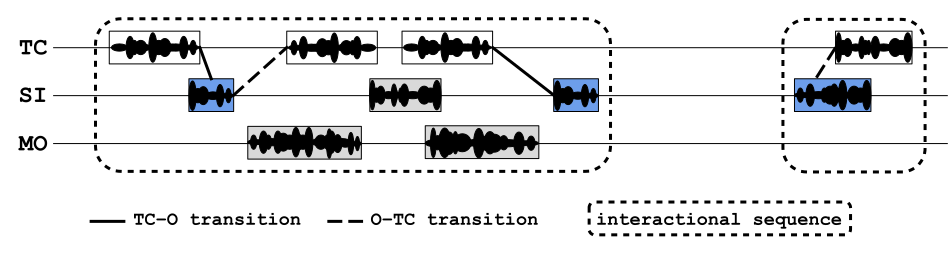
\includegraphics[width=1\linewidth]{Tseltal-CLE_files/TseltalCLE-TurnTimingIllustration} 

}

\caption{Illustration of an annotated audio clip including the target child (TC), an older sister (SI), and mother (MO). Transitions between the target child and others are marked with solid and dashed lines. Interactional sequences are boxed in with dotted lines. Box color indicates TCDS (blue) and ODS (light gray).}\label{fig:fig6}
\end{figure}

\subsection{Target-child-to-other turn transitions
(TC--O)}\label{target-child-to-other-turn-transitions-tco}

Contingent responses by or to the target child are likely to occur at
moments in which the child and another speaker are attentionally
aligned; the rate at which these responses is an index of the frequency
of these joint moments of high-quality linguistic evidence. We measured
two types of contingent responses: target-child-to-other and
other-to-target-child. We detect these contingent turn transitions based
on utterance onset/offset times and the annotations of intended
addressee for each non-target-child utterance
(\protect\hyperlink{fig6}{Figure 6}). If a child's vocalization is
followed by a target-child-directed utterance within -1000msec to
2000msec after its end (Casillas, Bobb, \& Clark, 2016; Hilbrink,
Gattis, \& Levinson, 2015), it is counted as a contingent response
(i.e., a TC--O transition). We use the same idea to find
other-to-target-child transitions (i.e., a target-child-directed
utterance followed by a target child vocalization with the same timing
restrictions). In our analysis, each target child vocalization can have
maximally have one prompt and one response, and each
target-child-directed utterance can maximally count once as a prompt and
once as a response (e.g., in a TC--O--TC sequence, the \enquote{O} is
both a response and a prompt). These timing restrictions are broadly
based on prior studies of infant and young children's spontaneous turn
taking (e.g., M. H. Bornstein, Putnick, Cote, Haynes, \& Suwalsky, 2015;
T. Broesch, Rochat, Olah, Broesch, \& Henrich, 2016; Casillas et al.,
2016; Hilbrink et al., 2015).

\begin{figure}
\centering
\includegraphics{Tseltal-CLE_files/figure-latex/fig7-1.pdf}
\caption{\label{fig:fig7}By-child estimates of target-child-to-other
contingent responses (left), other-to-target-child contingent responses
(middle), and the average duration of interactional sequences (right).
Each boxplot represents the variance across clips within the random
(dark purple; solid) or turn taking (light green; dashed) samples for
each child. Bands on the linear trends show 95\% CIs.}
\end{figure}

Other speakers responded contingently to the target children's
vocalizations at an average rate of 1.38 transitions per minute (median
= 0.40; range = 0--8.60; \protect\hyperlink{fig7}{Figure 7}). We modeled
TC--O transtions per minute in the random clips with a zero-inflated
negative binomial regression, excluding by-child intercepts of time of
day to achieve convergence. The rate at which target children heard
contingent responses from others was primarily influenced by factors
relating to the child's age. Older target children heard more contingent
responses then younger ones when there were more speakers present (B =
0.47, SD = 0.22, z = 2.11, p = 0.03). Also, as with the speech quantity
measures, older target children heard more contingent responses in the
mornings and evenings, while this effect was less pronounced for younger
ones (B = -6.46, SD = 2.56, z = -2.52, p = 0.01). There were no further
significant effects in the count or zero-inflation models.

\subsection{Other-to-target-child turn transitions
(O--TC)}\label{other-to-target-child-turn-transitions-otc}

The 10 Tseltal children responded contingently to others' target-child
vocalizations at an average rate of 1.17 transitions per minute (median
= 0.20; range = 0--8.80; \protect\hyperlink{fig7}{Figure 7}). We modeled
O--TC transtions per minute in the random clips with a zero-inflated
negative binomial regression, excluding by-child intercepts of time of
day to achieve convergence. The rate at which target children responded
contingently to others (O--TC turn transitions per minute) was similarly
influenced by child age and time of day: younger target children were
less likely than older ones to show peak response rates in the morning
and evening (B = -7.30, SD = 2.61, z = -2.80, p = 0.01). There were no
further significant effects in the count or zero-inflation models.

\subsection{Sequence duration}\label{sequence-duration}

We defined sequences of interaction as periods of contingent turn taking
with at least one target child vocalization and one
target-child-directed prompt or response from another speaker. To detect
sequences of interaction, we used the same mechanism as before to detect
contingent TC--O and O--TC transitions, but also allowed for speakers to
continue with multiple vocalizations in a row (e.g., TC--O--O--TC--OTH;
\protect\hyperlink{fig6}{Figure 6}). We bounded sequences by the
earliest and latest vocalization for which there is no contingent prompt
or response, respectively. In our analysis, each target child
vocalization can only appear in one sequence. We modeled these sequence
durations in the random clips with negative binomial regression alone,
excluding by-child intercepts of time of day to achieve convergence.

We detected 311 interactional sequences in the 90 randomly selected
clips, with an average sequence duration of 10.13 seconds (median = 7;
range = 0.56--85.47; \protect\hyperlink{fig7}{Figure 7}). The average
number of child vocalizations within these sequences was 3.75 (range =
1--29; median = 3). None of the predictors significantly impacted
sequence duration (all \emph{p} \textgreater{} 0.09).

\subsection{Peak interaction}\label{peak-interaction}

As expected, the high-quality turn taking clips featured a much higher
rate of contingent turn transitions: the average TC--O transition rate
was 7.73 transitions per minute (\textasciitilde{}5.5x the random sample
rate; median = 7.80; range = 0--25) and the average O--TC rate was 7.56
transitions per minute (\textasciitilde{}6.5x the random sample rate;
median = 6.20; range = 0--26). The interactional sequences were also
slightly longer on average: 12.27 seconds (\textasciitilde{}1.2x the
random sample rate; median = 8.10; range = 0.55--61.22). Crucially,
children also heard much more TCDS in the turn-taking clips---13.28
min/hr (nearly 4x the random sample rate; median = 13.65; range =
7.32--20.19)---while also hearing less ODS---11.93 min/hr (nearly half
the random sample rate; median = 10.18; range = 1.37--24.42).

We modeled each of these speech environment measures with parallel
models to those used for the random sample above, though with no
zero-inflation parameter for TCDS, TC--O, and O--TC rates because these
extra-zero cases don't exist in the manually selected turn-taking clips.
The impact of child age, time of day, household size, and number of
speakers was qualitatively similar (see \protect\hyperlink{fig3}{Figures
3}, \protect\hyperlink{fig4}{4}, and \protect\hyperlink{fig6}{6})
between the randomly selected clips and the turn taking clips with the
following exceptions: children heard significantly less ODS with age (B
= -0.47, SD = 0.20, z = -2.39, p = 0.02), the presence of more speakers
significantly decreased children's response rate to other's
vocalizations (B = -0.26, SD = 0.12, z = -2.19, p = 0.03), and
children's interactional sequences were shorter for older children (B =
-0.24, SD = 0.10, z = -2.42, p = 0.02), shorter for children in large
households (B = -0.21, SD = 0.10, z = -2.25, p = 0.02), and longer
during the mornings and evenings (B = 2.76, SD = 1.11, z = 2.50, p =
0.01). Full model outputs can be viewed in the Supplementary Materials.

\subsubsection{Peak minutes in the day}\label{peak-minutes-in-the-day}

Now knowing the interactional timing characteristics of the
\enquote{high} turn-taking clips, we looked for similarly
temporally-contingent 1-minute sections of interaction in the random
samples in order to estimate the number of high interactivity minutes in
the whole day. To do this, we scanned each 60-second window (e.g., 0--60
sec, 1--61 sec, etc.) of each random clip and recorded the observed
turn-transition rate. We then compared the resulting 1-minute transition
rates to those typical for the high turn taking sample.

Only 6 of the 10 children showed at least one minute of their random
sample that equalled or exceeded the average contingent transition rate
(12.89 transitions/min), and 7 of the 10 children showed at least one
minute equalling or exceeding their \emph{own} average turn transition
rate from their turn-taking sample. Across the 6 children who did show
turn-taking \enquote{peaks} in their random data, peak periods were
relatively long, at an average of 88.95 seconds (median = 90.67 seconds;
range = 71--103 seconds). Assuming approximately 14 waking hours (Hart
\& Risley, 1995), we therefore very roughly estimate that the Tseltal
child spends an average of 116.85 minutes (1.95 hours) in high
turn-taking, dyadic interaction during their day. Importantly, however,
the range in the quantity of high turn-taking interaction varies
enormously across children, starting at just a few minutes per day and
topping out at more than 489.69 minutes (8.16 hours) in our sample. Much
more data, particularly from other Tseltal children in this age range,
is required to get a stable estimate of peak minutes in the day.

\subsection{Vocal maturity}\label{vocal-maturity}

Tseltal children's vocalizations appear to follow the normative
benchmarks for productive speech development, as typically characterized
by the onset of new production features. Decades of research in
post-industrial, typically Western populations has shown that,
typically, children begin producing non-canonical babbles around 0;2,
with canonical babbling appearing sometime around 0;7, first words
around 1;0, with first multi-word utterances appearing just after 1;6
(Fine \& Lieven, 1993; Frank et al., in preparation; P. K. Kuhl, 2004;
Slobin, 1970; Tomasello \& Brooks, 1999; Warlaumont \& Finnegan, 2016;
Warlaumont, Richards, Gilkerson, \& Oller, 2016). These benchmarks are
mirrored in the Tseltal children's vocalizations, which are summarized
in \protect\hyperlink{fig9}{Figure 9} based on all annotated
vocalizations from the random, turn-taking, and high vocal activity
samples (N = 4725 vocalizations). There is a decline in the use of
non-canonical babble and an accompanying increase in the use of
canonical babble from 0;6 to 1;0. Recognizable words are observed for
every child from age 11;0 and older. Multi-word utterances appear in all
recordings at 1;2 and later, making up 45\% of the oldest child's (3;0)
vocalizations.

\begin{figure}
\centering
\includegraphics{Tseltal-CLE_files/figure-latex/fig9-1.pdf}
\caption{\label{fig:fig9}Proportion of vocalization types used by children
across age (NCB = Non-canonical babble, CB = Canonical babble, SW =
single word utterance, MW = multi-word utterance).}
\end{figure}

These data are also consistent with usage statistics of speech-like
vocalizations by English-acquiring infants (Oller, 1980; Warlaumont \&
Finnegan, 2016; Warlaumont et al., 2016). Between 2 and 14 months, these
Tseltal children demonstrated a large increase in the proportion of
speech-like vocalizations (canonical babbling and lexical speech): from
9\% before 0;6 to 58\% between 0;10 and 1;2. Around age 1;0, their use
of speech-like vocalizations (58\%) is nearly identical to that
estimated by Warlaumont et al. (2016) for American children around age
1;0 in a variable SES sample (\textasciitilde{}60\%).\footnote{Speech-like
  vs.~non-speech-like comparisons are limited to age 1;6 in the ACLEW
  Annotation Scheme.}

\section{Discussion}\label{disc}

We analyzed 10 Tseltal Mayan children's speech environments in order to
estimate how often they have the opportunity to attend and respond to
speech directed to them. We also investigated how these speech
environment characteristics changed (or stayed stable) across different
ages, household sizes, time of day, and number of speakers present. To
achieve representative estimates, we sampled audio segments randomly
from each child's daylong recording, but we show that most of the same
general patterns hold up during the \enquote{peak} turn-taking moments
of the day as well. Finally, we roughly estimated the number of
\enquote{high interactivity} minutes Tseltal children encounter on a
typical day and demonstrated that, despite the relatively small quantity
of CDS, children's early vocal development was on-par with norms built
from WEIRD children's data. These findings, which use a new methodology
(i.e., daylong recordings with multiple sample types), partly replicate
estimates of child language input and development in previous
ethnographic and psycholinguistic work on Yucatec and Tseltal Mayan
communities (Brown, 1997, 1998c, 2011, Tseltal: 2014; Shneidman, 2010;
Yucatec: Shneidman, Arroyo, Levine, \& Goldin-Meadow, 2012). In what
follows we briefly review each of the predictions made at the outset of
the paper.

\subsection{How much directed speech do Tseltal children
hear?}\label{how-much-directed-speech-do-tseltal-children-hear}

The bulk of our analyses were aimed at understanding how much speech
Tseltal children hear: we wanted to know how often they are directly
spoken to and how often they might be able to listen to other-directed
speech around them. As suggested by prior work, the children were only
infrequently directly spoken to: an average of 3.63 minutes per hour in
the random sample. Compared to other studies based on daylong
recordings, the Tseltal average TCDS rate is approximately a third of
that found for North American children (Bergelson et al., 2019), but is
comparable to that for Tsimane children (Scaff et al., in preparation).
The CDS estimates also fall almost precisely in-line with those based on
short-format recordings in a Yucatec Mayan village (Shneidman, 2010;
Shneidman et al., 2012).

A novel contribution of this study is that we also included interactive
measures to describe how often children were directly engaged with an
interlocutor, either as a responder or as an addressee being responded
to. We found that children's vocalizations were responded to at a rate
of 1.38 speaker transitions per minute and that children responded to
others' child-directed vocalizations at a rate of 1.17 transitions per
minute. Prior work from a number of different domains suggests that
contingent interaction (and the joint attention that likely accompanies
it) is an ideal context for language learning since the child and
interlocutor's coordinated attentional states decrease referential
uncertainty, are a source of dynamic feedback, and can spur more
interactions in the near future (M. H. Bornstein et al., 2015; T.
Broesch et al., 2016; Romeo et al., 2018; Warlaumont \& Finnegan, 2016;
Warlaumont et al., 2016). Because our measure is a novel one, we cannot
directly compare Tseltal children's data with those of children growing
up in other communities. That said, 1.38 and 1.17 transitions per minute
suggests that contingent responses---more so than speech directly
addressed to the child---are rare across children's day. Importantly,
however, this may be due to the fact that children did not vocalize very
often.

Preliminary analyses of children's vocal maturity showed that, on
average, children only produced 472.50 vocalizations (many of which were
crying, laughter, and non-canonical babble) during the entire 1-hour of
clips sampled from their daylong recordings. This explanation resonates
with the fact that, despite the low frequency of contingent turn-taking
in the random sample, interactional sequences were fairly long: 10.13
seconds. During these long sequences, children tended to only vocalize
3.75 times, meaning that many of children's dyadic interactional
sequences are marked by longer streams of directed input from another
speaker, interspersed with only occasional responses from the child.
Interactional peaks with contingent turn-taking \emph{do} occur in the
data, only rarely; our rough estimate is that Tseltal children
participate in approximately 100.16 minutes of such interaction during a
12-hour waking day, most of which come in bursts of \textasciitilde{}53
seconds long.

In sum, our results confirm prior claims that Tseltal children, like
other Mayan children, are not often directly spoken to. When they are,
much of their speech comes in interactional sequences in which children
only play a minor part---directly contingent turn transitions between
children and their interlocutors are relatively rare. However, we
estimate that the average child under age 3;0 experiences more than one
cumulative hour of high-intensity contingent interaction with CDS per
day. If child-directed speech quantity linearly feeds language
development (such that more input begets more output), then the
estimates presented here would lead us to expect that Tseltal children
are delayed in their language development, at least relative to North
American children. However, our initial analyses of early vocal
development suggest that Tseltal children, though they may not vocalize
often, demonstrate vocal maturity comparable to children from societies
in which CDS is known to be more frequent (Braine \& Bowerman, 1976;
Fine \& Lieven, 1993; Frank et al., in preparation; P. K. Kuhl, 2004;
Oller, 1980; Tomasello \& Brooks, 1999; Warlaumont \& Finnegan, 2016;
Warlaumont et al., 2016). How do Tseltal children manage this feat?

\subsubsection{Other-directed speech}\label{other-directed-speech}

One proposal is that Mayan children become experts at learning from
observation during their daily interactions (de León, 2011; Rogoff et
al., 2003; Shneidman, 2010; Shneidman et al., 2012), thereby bridging
the \enquote{gap} otherwise left by the lower rate of CDS. In the
randomly selected clips, children were within hearing distance of
other-directed speech for an average of 21.05 minutes per hour. That is
substantially more than the \textasciitilde{}7 minute per hour heard by
North American children (Bergelson et al., 2019), but comparable to the
\textasciitilde{}10 minutes per hour heard by Tsimane children (Scaff et
al., in preparation). The large quantity of other-directed speech is
likely due to the fact that Tseltal children (like Tsimane children)
tend to live in households with more people compared to North American
children (Bergelson et al., 2018).

In our data, the presence of more speakers was associated with
significantly more other-directed speech, both based on the number of
individual voices present in the clip and on the number of people living
in the household (for younger children). In comparison, children also
heard more CDS when more speakers were present, but the effect was much
weaker (0.2440 vs.~1.05622 more minutes per hour per speaker unit). This
finding rings true with Brown's (2011, 2014) claim that Tseltal is a
non-child-centric language community; the presence of more people
somewhat increases talk to the child but really primarily increases talk
amongst the other speakers. However, given that this increase in the
number of speakers and amount of talk is also associated with an
increase in the amount of overlapping speech (Cristia, Ganesh, Casillas,
\& Ganapathy, 2018), we suggest that attention to other-directed speech
is at least not the only learning mechanism needed to explain the
robustness of early vocal development in Tseltal. Furthermore, just
because speech is hearable does not mean children are attending to it.
Follow-up work on the role of other-directed speech in children's speech
development would need to clarify what constitutes viable
\enquote{listened to} speech by the child.

\subsubsection{Increased CDS with age}\label{increased-cds-with-age}

Another possibility is that CDS increases rapidly with child age (and
vocalization competence). Combined with the idea that very early
vocalizations follow a relatively species-specific, pre-programmed path
that is then modulated by caregiver response and other factors (Oller,
1980; Oller, Griebel, \& Warlaumont, 2016; Warlaumont \& Finnegan, 2016;
Warlaumont et al., 2016), a dramatic increase in directed speech with
age might be expected. In her longitudinal studies of Yucatec Mayan
children, Shneidman (2012) found that CDS increased significantly with
age, from 55 utterances in an hour to 209 between 13 and 35 months. Her
analyses show that most of the increase in CDS comes from other children
speaking to the target child. Her findings are consistent with other
reports that Mayan children are more often cared for by their older
siblings from later infancy onward (2011, 2014). In our data, however,
age effects were limited, and CDS from children was relatively rare
(\textasciitilde{}10\%) all the way up through age 3;0.

Child age alone had very little overall effect on the speech environment
measures. In the random sample it was, at most, associated with marginal
increases in TC--O transition rate, O--TC transition rate, and sequence
duration. All other significant effects involving age related to the
time of day measure, which is discussed below.

The non-increase in CDS with age may be due to the fact CDS from other
children was infrequent in our data (cf. Shneidman \& Goldin-Meadow,
2012). The relative lack of CDS may be due to the fact that: (a) the
children were relatively young and so spent much of their time with
their mothers, (b) these particular children did not have many older
siblings, and (c) in the daylong recording context more adults were
present to talk to each other than would be typical in a short-format
recording (the basis for previous estimates). We conclude, from these
findings, that an increase in CDS cannot explain the robust pattern of
Tseltal vocal development either.

\subsubsection{Learning from short periods of
interaction}\label{learning-from-short-periods-of-interaction}

A third possibility is that these children learn effectively from short,
routine language encounters. Bursty input appears to be the norm across
a number of linguistic and interactive scales (e.g., Abney et al., 2017;
Blasi et al., in preparation), and experiment-based work suggests that
children can benefit from massed presentation of new information (Schwab
\& Lew-Williams, 2016). We propose two mechanisms through which Tseltal
children might capitalize on the distribution of speech input in their
environment: they experience most language input during routine
activities and they can consolidate experienced input during the
downtime between interactive peaks. Neither of these mechanisms are
proposed to be particular to Tseltal children, but might be employed to
explain their efficient learning.

Tseltal children's linguistic input is not uniformly distributed over
the day: all five measures of children's linguistic environment were
more likely to occur in the mornings and afternoons than around midday,
though younger children showed this pattern more robustly than older
children. We had predicted a dip in linguistic input around midday
because household members tend to disperse after breakfast to do their
daily work before returning for another late afternoon meal. Young
children, who are typically carried by their mothers for the majority of
the day, followed this pattern more strongly than older children, who
may have been more free to seek out interactions between mealtimes. A
similar midday dip has been previously found for North American
children's daylong recordings (Greenwood et al., 2011; Soderstrom \&
Wittebolle, 2013), suggesting that non-uniform distributions of
linguistic input may be the norm for children in a variety of different
cultural-economic contexts. Our paper is the first to show that those
time of day effects change with age in the first few years on a number
of speech environment features (TCDS, TC--O transitions, O--TC
transitions, and (marginally) ODS).

Our impression from having transcribed these data is that the time of
day effects likely arise from the activities that typically occur in the
mornings and afternoons---meal preparation and dining times in
particular---while napping could contribute to the midday dip
(Soderstrom \& Wittebolle, 2013). Indeed, time of day effects in daylong
recordings at Canadian homes and daycares were substantially weakened
when naptimes were excluded from the analysis (Soderstrom \& Wittebolle,
2013). However, in the same Canadian data, the highest density speech
input came during storytime and organized playtime (e.g., sing-alongs,
painting), while mealtime was associated with less speech input. We
expect that follow-up research which tracks activities in the Tseltal
data will lead to very different conclusions: storytime and organized
playtime are vanishingly rare in this non-child-centric community, and
mealtime may represent a time of routine and rich linguistic experience.
In both cases, however, the underlying association with activity (not
hour) implies the possibility for action routines that may help children
optimally extract information about what they will encounter and what
they are expected to do in response, even over short periods (Bruner,
1983; Ferrier, 1978; tamis2018routine; Nelson, 1985; Shatz, 1978; Snow
\& Goldfield, 1983).

A more speculative possibility is that Tseltal children learn language
on a natural input-consolidation cycle: the rarity of interactional
peaks throughout the day may be complemented by an opportunity to
consolidate new information. Sleep has been shown to benefit language
learning tasks in both adults (Dumay \& Gaskell, 2007; Frost \&
Monaghan, 2017; Mirković \& Gaskell, 2016) and children (Gómez, Bootzin,
\& Nadel, 2006; Horváth, Liu, \& Plunkett, 2016; Hupbach, Gomez,
Bootzin, \& Nadel, 2009; Williams \& Horst, 2014), including word
learning, phonotactic constraints, and syntactic structure. Our
impression, both from the recordings and informal observations made
during visits to the community, is that young Tseltal children take
frequent naps, particularly at younger ages when they spend much of
their day wrapped within the shawl on their mother's back. Mayan
children tend to pick their own resting times (i.e., there are no
formalized ``sleep'' times, even at bedtime Morelli, Rogoff, Oppenheim,
\& Goldsmith, 1992), and Mayan mothers take special care to keep infants
in a calm and soothing environment in the first few months of life
(Brazelton, 1972; e.g., de León, 2000; Pye, 1992; E. Z. Vogt, 1976).
There is little quantitative data on Mayan children's daytime and
nighttime sleeping patterns, but one study estimates that Yucatec Mayan
children between 0;0 and 2;0 sleep or rest nearly 15\% of the time
between morning and evening (Gaskins, 2000), again, at times that suited
the child (Morelli et al., 1992). If Tseltal children's interactional
peaks are bookended by short naps, it could contribute to efficient
consolidation of new information encountered. How often Tseltal children
sleep, how deeply, and how their sleeping patterns may relate to their
linguistic development is an important topic for future research.

\subsection{Limitations and Future Work}\label{disc-limfut}

The current findings are based on a cross-sectional analysis of only 10
children. From each child, we have manually only analyzed a total of 1
of the 9--11 recording hours. The findings only take into account verbal
input; the photo-linked audio we produce is not sufficient to analyze
gaze and gestural behavior (Brown, 2014). In short, more data, and more
kinds of data are needed to enrich this initial description of Tseltal
children's early language environments. We have also used vocal maturity
as an index of linguistic development in the current study, but further
analysis of these children's receptive and productive lexical,
morphological, and syntactic knowledge, including experiment and
questionnaire based measures that build on past linguistic work (Brown,
1997, 1998b, 1998c, 1998a, 2011, 2014; Brown \& Gaskins, 2014) is needed
to establish trajectory of early language development in Tseltal
(Casillas et al., 2017a). To fully understand the extent to which
language learning mechanisms are shared across ethnolinguistically
diverse samples we cannot simply continue to compare developmental
benchmarks. More promising long-term approaches include a focus on how
within-community differences and/or cross-linguistic differences for
related languages drive variation in learning (e.g., Pye, 2017;
Weisleder \& Fernald, 2013). The current analyses are based on a corpus
that is under active development. As new data are added, up-to-date
versions of the same analyses will be available on the same page where
the current data and analysis scripts can be found: ADD-URL.

\subsection{Conclusion}\label{disc-conclusion}

Based on the current data, we estimate that Tseltal children hear an
average of 3.6 minutes of directed speech per hour. Contingent
turn-taking is relatively rare throughout their day, and high-intensity
interactive input comes in short bursts, typically in the mornings and
early evenings for younger children. Despite this relatively small
quantity of directed speech, Tseltal children's vocal maturity looks
on-track with estimates based on WEIRD populations, in which children
typically experience more child-directed speech. Our findings by and
large replicate the descriptions put forth by linguistic anthropologists
who have worked with Mayan communities for many decades. The real puzzle
is then how Tseltal children efficiently extract information from their
linguistic environments. We reviewed several proposals and outlined
directions for future work. In our view, a promising avenue for
continued research is to more closely investigate the
activity/time-of-day effects and a possible input-consolidation cycle
for language exposure in early infancy. By better understanding how
Tseltal children learn language, we hope to uncover some of the ways in
which human learning mechanisms are adaptive to the thousands of
ethnolinguistic environments in which children develop.

\section{Acknowledgements}\label{acknowledgements}

\textbf{Needs to be adjusted} This work would not be possible without
the efforts of Rebeca, Beti, Xun, their cousin, and Antun. We are
enormously grateful to the participating families for sharing their
lives with us. We also thank the community and community leaders in
Tenejapa for supporting our work. Thanks too, to Maartje Weenink and
Daphne Jansen, who have spent many hours identifying clips for
transcription and errors in annotation. This work was supported by a NWO
Veni Innovational Scheme grant (275-89-033) to MC and by an ERC Advanced
Grant (269484 INTERACT) project to SCL. This manuscript was written
using the papaja library in RStudio (Aust \& Barth, 2018; RStudio Team,
2016).

\newpage

\section{References}\label{refs}

\begingroup
\setlength{\parindent}{-0.5in} \setlength{\leftskip}{0.5in}

\hypertarget{refs}{}
\hypertarget{ref-abney2017time}{}
Abney, D. H., Smith, L. B., \& Yu, C. (2017). It's time: Quantifying the
relevant time scales for joint attention. In G. Gunzelmann, A. Howes, T.
Tenbrink, \& E. Davelaar (Eds.), \emph{Proceedings of the 39th annual
meeting of the cognitive science society} (pp. 1489--1494). London, UK.

\hypertarget{ref-R-papaja}{}
Aust, F., \& Barth, M. (2018). \emph{papaja: Create APA manuscripts with
R Markdown}. Retrieved from \url{https://github.com/crsh/papaja}

\hypertarget{ref-bates1997inseparability}{}
Bates, E., \& Goodman, J. C. (1997). On the inseparability of grammar
and the lexicon: Evidence from acquisition, aphasia, and real-time
processing. \emph{Language and Cognitive Processes}, \emph{12}(5--6),
507--584.
doi:\href{https://doi.org/doi.org/10.1080/016909697386628}{doi.org/10.1080/016909697386628}

\hypertarget{ref-bergelson2018day}{}
Bergelson, E., Amatuni, A., Dailey, S., Koorathota, S., \& Tor, S.
(2018). Day by day, hour by hour: Naturalistic language input to
infants. \emph{Developmental Science}, \emph{XX}, XX--XX.

\hypertarget{ref-bergelsoncasillas2019what}{}
Bergelson, E., Casillas, M., Soderstrom, M., Seidl, A., Warlaumont, A.
S., \& Amatuni, A. (2019). What do north american babies hear? A
large-scale cross-corpus analysis. \emph{Developmental Science},
\emph{22}(1), e12724.
doi:\href{https://doi.org/doi:10.1111/desc.12724}{doi:10.1111/desc.12724}

\hypertarget{ref-blasiIPhuman}{}
Blasi, D., Schikowski, R., Moran, S., Pfeiler, B., \& Stoll, S. (in
preparation). Human communication is structured efficiently for first
language learners: Lexical spikes.

\hypertarget{ref-bornstein2015mother}{}
Bornstein, M. H., Putnick, D. L., Cote, L. R., Haynes, O. M., \&
Suwalsky, J. T. D. (2015). Mother-infant contingent vocalizations in 11
countries. \emph{Psychological Science}, \emph{26}(8), 1272--1284.

\hypertarget{ref-braine1976childrens}{}
Braine, M. D. S., \& Bowerman, M. (1976). Children's first word
combinations. \emph{Monographs of the Society for Research in Child
Development}, 1--104.

\hypertarget{ref-brazelton1972implications}{}
Brazelton, T. B. (1972). Implications of infant development among the
mayan indians of mexico. \emph{Human Development}, \emph{15}(2),
90--111.

\hypertarget{ref-brinchmann2019direct}{}
Brinchmann, E. I., Braeken, J., \& Lyster, S.-A. H. (2019). Is there a
direct relation between the development of vocabulary and grammar?
\emph{Developmental Science}, \emph{22}(1), e12709.

\hypertarget{ref-broesch2016similarities}{}
Broesch, T., Rochat, P., Olah, K., Broesch, J., \& Henrich, J. (2016).
Similarities and differences in maternal responsiveness in three
societies: Evidence from Fiji, Kenya, and the United States. \emph{Child
Development}, \emph{87}(3), 700--711.

\hypertarget{ref-R-glmmTMB}{}
Brooks, M. E., Kristensen, K., van Benthem, K. J., Magnusson, A., Berg,
C. W., Nielsen, A., \ldots{} Bolker, B. M. (2017a). glmmTMB balances
speed and flexibility among packages for zero-inflated generalized
linear mixed modeling. \emph{The R Journal}, \emph{9}(2), 378--400.
Retrieved from
\url{https://journal.r-project.org/archive/2017/RJ-2017-066/index.html}

\hypertarget{ref-brooks2017modeling}{}
Brooks, M. E., Kristensen, K., van Benthem, K. J., Magnusson, A., Berg,
C. W., Nielsen, A., \ldots{} Bolker, B. M. (2017b). Modeling
zero-inflated count data with glmmTMB. \emph{bioRxiv}.
doi:\href{https://doi.org/10.1101/132753}{10.1101/132753}

\hypertarget{ref-brown1997isolating}{}
Brown, P. (1997). Isolating the cvc root in tzeltal mayan: A study of
children's first verbs. In E. V. Clark (Ed.), \emph{Proceedings of the
28th annual child language research forum} (pp. 41--52). Stanford, CA:
CSLI Publications/University of Chicago Press.

\hypertarget{ref-brown1998childrens}{}
Brown, P. (1998a). Children's first verbs in tzeltal: Evidence for an
early verb category. \emph{Linguistics}, \emph{36}(4), 713--753.

\hypertarget{ref-brown1998conversational}{}
Brown, P. (1998b). Conversational structure and language acquisition:
The role of repetition in tzeltal adult and child speech. \emph{Journal
of Linguistic Anthropology}, \emph{2}, 197--221.
doi:\href{https://doi.org/10.1525/jlin.1998.8.2.197}{10.1525/jlin.1998.8.2.197}

\hypertarget{ref-brown1998early}{}
Brown, P. (1998c). Early tzeltal verbs: Argument structure and argument
representation. In E. V. Clark (Ed.), \emph{Proceedings of the 29th
annual stanford child language research forum} (pp. 129--140). Stanford,
CA: CSLI Publications.

\hypertarget{ref-brown2011cultural}{}
Brown, P. (2011). The cultural organization of attention. In A. Duranti,
E. Ochs, \& and B.B. Schieffelin (Eds.), \emph{Handbook of language
socialization} (pp. 29--55). Malden, MA: Wiley-Blackwell.

\hypertarget{ref-brown2014interactional}{}
Brown, P. (2014). The interactional context of language learning in
tzeltal. In I. Arnon, M. Casillas, C. Kurumada, \& B. Estigarribia
(Eds.), \emph{Language in interaction: Studies in honor of eve v. clark}
(pp. 51--82). Amsterdam, NL: John Benjamins.

\hypertarget{ref-brownIPchildrearing}{}
Brown, P., \& Casillas, M. (in press). Childrearing through social
interaction on rossel island, png. In A. J. Fentiman \& M. Goody (Eds.),
\emph{Esther goody revisited: Exploring the legacy of an original
inter-disciplinarian} (pp. XX--XX). New York, NY: Berghahn.

\hypertarget{ref-brown2014language}{}
Brown, P., \& Gaskins, S. (2014). Language acquisition and language
socialization. In N. J. Enfield, P. Kockelman, \& J. Sidnell (Eds.),
\emph{Handbook of linguistic anthropology} (pp. 183--222). Cambridge,
UK: Cambridge University Press.

\hypertarget{ref-bruner1983childs}{}
Bruner, J. (1983). \emph{Child's talk}. Oxford: Oxford University Press.

\hypertarget{ref-butterworth2003pointing}{}
Butterworth, G. (2003). Pointing is the royal road to language for
babies. In S. Kita (Ed.), \emph{Pointing} (pp. 17--42). Psychology
Press.

\hypertarget{ref-cartmill2013quality}{}
Cartmill, E. A., Armstrong, B. F., Gleitman, L. R., Goldin-Meadow, S.,
Medina, T. N., \& Trueswell, J. C. (2013). Quality of early parent input
predicts child vocabulary 3 years later. \emph{Proceedings of the
National Academy of Sciences}, \emph{110}(28), 11278--11283.

\hypertarget{ref-casillas2016turn}{}
Casillas, M., Bobb, S. C., \& Clark, E. V. (2016). Turn taking, timing,
and planning in early language acquisition. \emph{Journal of Child
Language}, \emph{43}, 1310--1337.

\hypertarget{ref-Casillas-HB}{}
Casillas, M., Brown, P., \& Levinson, S. C. (2017a). Casillas HomeBank
corpus.

\hypertarget{ref-casillas2017ACLEWDAS}{}
Casillas, M., Bunce, J., Soderstrom, M., Rosemberg, C., Migdalek, M.,
Alam, F., \ldots{} Garrison, H. (2017b). Introduction: The aclew das
template {[}training materials{]}. Retrieved from
\url{https://osf.io/aknjv/}

\hypertarget{ref-cooper1990preference}{}
Cooper, R. P., \& Aslin, R. N. (1990). Preference for infant-directed
speech in the first month after birth. \emph{Child Development},
\emph{20}(4), 477--488.
doi:\href{https://doi.org/10.1016/S0163-6383(97)90037-0}{10.1016/S0163-6383(97)90037-0}

\hypertarget{ref-cristia2013input}{}
Cristia, A. (2013). Input to language: The phonetics and perception of
infant-directed speech. \emph{Language and Linguistics Compass},
\emph{7}(3), 157--170.
doi:\href{https://doi.org/10.1111/lnc3.12015}{10.1111/lnc3.12015}

\hypertarget{ref-cristia2017child}{}
Cristia, A., Dupoux, E., Gurven, M., \& Stieglitz, J. (2017).
Child-directed speech is infrequent in a forager-farmer population: A
time allocation study. \emph{Child Development}, XX--XX.
doi:\href{https://doi.org/10.1111/cdev.12974}{10.1111/cdev.12974}

\hypertarget{ref-cristia2018talker}{}
Cristia, A., Ganesh, S., Casillas, M., \& Ganapathy, S. (2018). Talker
diarization in the wild: The case of child-centered daylong
audio-recordings. \emph{Proceedings of Interspeech 2018}.
doi:\href{https://doi.org/doi:10.21437/Interspeech.2018-2078}{doi:10.21437/Interspeech.2018-2078}

\hypertarget{ref-deleon2000emergent}{}
de León, L. (2000). The emergent participant: Interactive patterns in
the socialization of Tzotzil (Mayan) infants. \emph{Journal of
Linguistic Anthropology}, \emph{8}(2), 131--161.

\hypertarget{ref-deleon2011language}{}
de León, L. (2011). Language socialization and multiparty participation
frameworks. In A. Duranti, E. Ochs, \& and B.B. Schieffelin (Eds.),
\emph{Handbook of language socialization} (pp. 81--111). Malden, MA:
Wiley-Blackwell.
doi:\href{https://doi.org/10.1002/9781444342901.ch4}{10.1002/9781444342901.ch4}

\hypertarget{ref-dumay2007sleep}{}
Dumay, N., \& Gaskell, M. G. (2007). Sleep-associated changes in the
mental representation of spoken words. \emph{Psychological Science},
\emph{18}(1), 35--39.

\hypertarget{ref-ferrier1978some}{}
Ferrier, L. J. (1978). Some observations of error in context. In N.
Waterson \& C. Snow (Eds.), \emph{The development of communication} (pp.
301--309). New York: Wiley Press.

\hypertarget{ref-pine1993reanalysing}{}
Fine, J. M., \& Lieven, E. V. M. (1993). Reanalysing rote-learned
phrases: Individual differences in the transition to multi-word speech.
\emph{Journal of Child Language}, 551--571.

\hypertarget{ref-frankIPvariability}{}
Frank, M. C., Braginsky, M., Marchman, V. A., \& Yurovsky, D. (in
preparation). \emph{Variability and consistency in early language
learning: The Wordbank project}. XX. Retrieved from
\url{https://langcog.github.io/wordbank-book/}

\hypertarget{ref-frost2017sleep}{}
Frost, R. L. A., \& Monaghan, P. (2017). Sleep-driven computations in
speech processing. \emph{PloS One}, \emph{12}(1), e0169538.
doi:\href{https://doi.org/doi:10.1371/journal.pone.0169538}{doi:10.1371/journal.pone.0169538}

\hypertarget{ref-gaskins1996how}{}
Gaskins, S. (1996). How Mayan parental theories come into play.
\emph{Parents' Cultural Belief Systems: Their Origins, Expressions, and
Consequences}, 345--363.

\hypertarget{ref-gaskins1999childrens}{}
Gaskins, S. (1999). Children's daily lives in a Mayan village: A case
study of culturally constructed roles and activities. In A. Göncü (Ed.),
\emph{Children's engagement in the world: Sociocultural perspectives}
(pp. 25--60). Oxford: Berg.

\hypertarget{ref-gaskins2000childrens}{}
Gaskins, S. (2000). Children's daily activities in a Mayan village: A
culturally grounded description. \emph{Cross-Cultural Research},
\emph{34}(4), 375--389.

\hypertarget{ref-gaskins2006cultural}{}
Gaskins, S. (2006). Cultural perspectives on infant--caregiver
interaction. In N. J. Enfield \& S. Levinson (Eds.), \emph{Roots of
human sociality: Culture, cognition and interaction} (pp. 279--298).
Oxford: Berg.

\hypertarget{ref-goldberg2003constructions}{}
Goldberg, A. E. (2003). Constructions: A new theoretical approach to
language. \emph{Trends in Cognitive Sciences}, \emph{7}(5), 219--224.

\hypertarget{ref-golinkoff2015baby}{}
Golinkoff, R. M., Can, D. D., Soderstrom, M., \& Hirsh-Pasek, K. (2015).
(Baby) talk to me: The social context of infant-directed speech and its
effects on early language acquisition. \emph{Current Directions in
Psychological Science}, \emph{24}(5), 339--344.

\hypertarget{ref-gomez2006naps}{}
Gómez, R. L., Bootzin, R. R., \& Nadel, L. (2006). Naps promote
abstraction in language-learning infants. \emph{Psychological Science},
\emph{17}(8), 670--674.

\hypertarget{ref-greenwood2011assessing}{}
Greenwood, C. R., Thiemann-Bourque, K., Walker, D., Buzhardt, J., \&
Gilkerson, J. (2011). Assessing children's home language environments
using automatic speech recognition technology. \emph{Communication
Disorders Quarterly}, \emph{32}(2), 83--92.
doi:\href{https://doi.org/10.1177/1525740110367826}{10.1177/1525740110367826}

\hypertarget{ref-hart1995meaningful}{}
Hart, B., \& Risley, T. R. (1995). \emph{Meaningful Differences in the
Everyday Experience of Young American Children}. Paul H. Brookes
Publishing.

\hypertarget{ref-henrich2010beyond}{}
Henrich, J., Heine, S. J., \& Norenzayan, A. (2010). Beyond WEIRD:
Towards a broad-based behavioral science. \emph{Behavioral and Brain
Sciences}, \emph{33}(2--3), 111--135.

\hypertarget{ref-hilbrink2015early}{}
Hilbrink, E., Gattis, M., \& Levinson, S. C. (2015). Early developmental
changes in the timing of turn-taking: A longitudinal study of
mother--infant interaction. \emph{Frontiers in Psychology},
\emph{6:1492}, 1--12.

\hypertarget{ref-hoff2003specificity}{}
Hoff, E. (2003). The specificity of environmental influence:
Socioeconomic status affects early vocabulary development via maternal
speech. \emph{Child Development}, \emph{74}(5), 1368--1378.

\hypertarget{ref-hoff2006social}{}
Hoff, E. (2006). How social contexts support and shape language
development. \emph{Developmental Review}, \emph{26}(1), 55--88.

\hypertarget{ref-horvath2016daytime}{}
Horváth, K., Liu, S., \& Plunkett, K. (2016). A daytime nap facilitates
generalization of word meanings in young toddlers. \emph{Sleep},
\emph{39}(1), 203--207.

\hypertarget{ref-hupbach2009nap}{}
Hupbach, A., Gomez, R. L., Bootzin, R. R., \& Nadel, L. (2009).
Nap-dependent learning in infants. \emph{Developmental Science},
\emph{12}(6), 1007--1012.

\hypertarget{ref-hurtado2008does}{}
Hurtado, N., Marchman, V. A., \& Fernald, A. (2008). Does input
influence uptake? Links between maternal talk, processing speed and
vocabulary size in spanish-learning children. \emph{Developmental
Science}, \emph{11}(6), F31--F39.
doi:\href{https://doi.org/10.1111/j.1467-7687.2008.00768.x\%5D}{10.1111/j.1467-7687.2008.00768.x{]}}

\hypertarget{ref-huttenlocher2010sources}{}
Huttenlocher, J., Waterfall, H., Vasilyeva, M., Vevea, J., \& Hedges, L.
V. (2010). Sources of variability in children's language growth.
\emph{Cognitive Psychology}, \emph{61}, 343--365.

\hypertarget{ref-kuhl2004early}{}
Kuhl, P. K. (2004). Early language acquisition: Cracking the speech
code. \emph{Nature Reviews Neuroscience}, \emph{5}(11), 831.

\hypertarget{ref-deleon1998emergent}{}
León, L. de. (1998). The emergent participant: Interactive patterns in
the socialization of Tzotzil (Mayan) infants. \emph{Journal of
Linguistic Anthropology}, \emph{8}(2), 131--161.

\hypertarget{ref-lieven1994crosslinguistic}{}
Lieven, E. V. M. (1994). Crosslinguistic and crosscultural aspects of
language addressed to children. In C. Gallaway \& B. J. Richards (Eds.),
\emph{Input and interaction in language acquisition} (pp. 56--73). New
York, NY, US: Cambridge University Press.
doi:\href{https://doi.org/10.1017/CBO9780511620690.005}{10.1017/CBO9780511620690.005}

\hypertarget{ref-lieven1997lexically}{}
Lieven, E. V. M., Pine, J. M., \& Baldwin, G. (1997). Lexically-based
learning and early grammatical development. \emph{Journal of Child
Language}, \emph{24}(1), 187--219.

\hypertarget{ref-liszkowski2012prelinguistic}{}
Liszkowski, U., Brown, P., Callaghan, T., Takada, A., \& De Vos, C.
(2012). A prelinguistic gestural universal of human communication.
\emph{Cognitive Science}, \emph{36}(4), 698--713.

\hypertarget{ref-manybabies2017}{}
ManyBabies Collaborative. (2017). Quantifying sources of variability in
infancy research using the infant-directed speech preference.
\emph{Advances in Methods and Practices in Psychological Science},
\emph{XX}, XX--XX.
doi:\href{https://doi.org/10.31234/osf.io/s98ab}{10.31234/osf.io/s98ab}

\hypertarget{ref-marchman2004language}{}
Marchman, V. A., Martínez-Sussmann, C., \& Dale, P. S. (2004). The
language-specific nature of grammatical development: Evidence from
bilingual language learners. \emph{Developmental Science}, \emph{7}(2),
212--224.

\hypertarget{ref-mirkovic2016does}{}
Mirković, J., \& Gaskell, M. G. (2016). Does sleep improve your grammar?
Preferential consolidation of arbitrary components of new linguistic
knowledge. \emph{PloS One}, \emph{11}(4), e0152489.

\hypertarget{ref-morelli1992cultural}{}
Morelli, G. A., Rogoff, B., Oppenheim, D., \& Goldsmith, D. (1992).
Cultural variation in infants' sleeping arrangements: Questions of
independence. \emph{Developmental Psychology}, \emph{28}(4), 604.

\hypertarget{ref-nelson1985making}{}
Nelson, K. (1985). \emph{Making sense: The acquisition of shared
meaning}. New York: Academic Press.

\hypertarget{ref-nielsen2017persistent}{}
Nielsen, M., Haun, D., Kärtner, J., \& Legare, C. H. (2017). The
persistent sampling bias in developmental psychology: A call to action.
\emph{Journal of Experimental Child Psychology}, \emph{162}, 31--38.

\hypertarget{ref-ochs1984language}{}
Ochs, E., \& Schieffelin, B. (1984). Language acquisition and
socialization: Three developmental stories and their implications. In R.
A. Schweder \& R. A. LeVine (Eds.), \emph{Culture theory: Essays on
mind, self, and emotion} (pp. 276--322). Cambridge University Press.

\hypertarget{ref-oller1980emergence}{}
Oller, D. K. (1980). The emergence of the sounds of speech in infancy.
In G. H. Yeni-Komshian, J. F. Kavanagh, \& C. A. Ferguson (Eds.),
\emph{Child phonology, volume 1: Production} (pp. 93--112). New York,
NY: Academic Press.

\hypertarget{ref-oller2016vocal}{}
Oller, D. K., Griebel, U., \& Warlaumont, A. S. (2016). Vocal
development as a guide to modeling the evolution of language.
\emph{Topics in Cognitive Science}, \emph{8}, 382--392.
doi:\href{https://doi.org/DOI:10.1111/tops.12198}{DOI:10.1111/tops.12198}

\hypertarget{ref-pye1986quiche}{}
Pye, C. (1986). Quiché Mayan speech to children. \emph{Journal of Child
Language}, \emph{13}(1), 85--100.

\hypertarget{ref-pye1992acquisition}{}
Pye, C. (1992). The acquisition of ki'che'. In D. I. Slobin (Ed.),
\emph{The crosslinguistic study of language acquisition, volume 3} (pp.
221--308). Hillsdale, NJ: Lawrence Erlbaum Associates.

\hypertarget{ref-pye2017comparative}{}
Pye, C. (2017). \emph{The comparative method of language acquisition
research}. University of Chicago Press.

\hypertarget{ref-R-base}{}
R Core Team. (2018). \emph{R: A language and environment for statistical
computing}. Vienna, Austria: R Foundation for Statistical Computing.
Retrieved from \url{https://www.R-project.org/}

\hypertarget{ref-ramirezesparza2014look}{}
Ramírez-Esparza, N., García-Sierra, A., \& Kuhl, P. K. (2014). Look
who's talking: Speech style and social context in language input to
infants are linked to concurrent and future speech development.
\emph{Developmental Science}, \emph{17}, 880--891.

\hypertarget{ref-rogoff1993guided}{}
Rogoff, B., Mistry, J., Göncü, A., Mosier, C., Chavajay, P., \& Heath,
S. B. (1993). Guided participation in cultural activity by toddlers and
caregivers. \emph{Monographs of the Society for Research in Child
Development}.

\hypertarget{ref-rogoff2003firsthand}{}
Rogoff, B., Paradise, R., Arauz, R. M., Correa-Chávez, M., \& Angelillo,
C. (2003). Firsthand learning through intent participation. \emph{Annual
Review of Psychology}, \emph{54}(1), 175--203.
doi:\href{https://doi.org/10.1146/annurev.psych.54.101601.145118}{10.1146/annurev.psych.54.101601.145118}

\hypertarget{ref-romeo2018beyond}{}
Romeo, R. R., Leonard, J. A., Robinson, S. T., West, M. R., Mackey, A.
P., Rowe, M. L., \& Gabrieli, J. D. E. (2018). Beyond the
30-million-word gap: Children's conversational exposure is associated
with language-related brain function. \emph{Psychological Science},
\emph{29}(5), 700--710.

\hypertarget{ref-rowe2008child}{}
Rowe, M. L. (2008). Child-directed speech: Relation to socioeconomic
status, knowledge of child development and child vocabulary skill.
\emph{Journal of Child Language}, \emph{35}(1), 185--205.

\hypertarget{ref-R-studio}{}
RStudio Team. (2016). \emph{RStudio: Integrated development environment
for r}. Boston, MA: RStudio, Inc. Retrieved from
\url{http://www.rstudio.com/}

\hypertarget{ref-salomo2013sociocultural}{}
Salomo, D., \& Liszkowski, U. (2013). Sociocultural settings influence
the emergence of prelinguistic deictic gestures. \emph{Child
Development}, \emph{84}(4), 1296--1307.

\hypertarget{ref-scaffIPlanguage}{}
Scaff, C., Stieglitz, J., Casillas, M., \& Cristia, A. (in preparation).
Language input in a hunter-forager population: Estimations from daylong
recordings.

\hypertarget{ref-schwab2016repetition}{}
Schwab, J. F., \& Lew-Williams, C. (2016). Repetition across successive
sentences facilitates young children's word learning.
\emph{Developmental Psychology}, \emph{52}(6), 879--886.

\hypertarget{ref-segal2015infant}{}
Segal, J., \& Newman, R. S. (2015). Infant preferences for structural
and prosodic properties of infant-directed speech in the second year of
life. \emph{Infancy}, \emph{20}(3), 339--351.
doi:\href{https://doi.org/10.1111/infa.12077}{10.1111/infa.12077}

\hypertarget{ref-shatz1978development}{}
Shatz, M. (1978). On the development of communicative understandings: An
early strategy for interpreting and responding to messages.
\emph{Cognitive Psychology}, \emph{10}, 271--301.

\hypertarget{ref-shneidman2010language}{}
Shneidman, L. A. (2010). \emph{Language input and acquisition in a Mayan
village} (PhD thesis). The University of Chicago.

\hypertarget{ref-shneidman2012language}{}
Shneidman, L. A., \& Goldin-Meadow, S. (2012). Language input and
acquisition in a Mayan village: How important is directed speech?
\emph{Developmental Science}, \emph{15}(5), 659--673.

\hypertarget{ref-shneidman2012counts}{}
Shneidman, L. A., Arroyo, M. E., Levine, S. C., \& Goldin-Meadow, S.
(2012). What counts as effective input for word learning? \emph{Journal
of Child Language}, \emph{40}(3), 672--686.

\hypertarget{ref-slobin1970universals}{}
Slobin, D. I. (1970). Universals of grammatical development in children.
In G. B. Flores d'Arcais \& W. J. M. Levelt (Eds.), \emph{Advances in
psycholinguistics} (pp. 174--186). Amsterdam, NL: North Holland
Publishing.

\hypertarget{ref-smithson2013generalized}{}
Smithson, M., \& Merkle, E. (2013). \emph{Generalized linear models for
categorical and continuous limited dependent variables}. CRC Press: Boca
Raton.

\hypertarget{ref-snow1983turn}{}
Snow, C. E., \& Goldfield, B. A. (1983). Turn the page please:
Situation-specific language acquisition. \emph{Journal of Child
Language}, \emph{10}(3), 551--569.

\hypertarget{ref-soderstrom2007beyond}{}
Soderstrom, M. (2007). Beyond babytalk: Re-evaluating the nature and
content of speech input to preverbal infants. \emph{Developmental
Review}, \emph{27}(4), 501--532.

\hypertarget{ref-soderstrom2013when}{}
Soderstrom, M., \& Wittebolle, K. (2013). When do caregivers talk? The
influences of activity and time of day on caregiver speech and child
vocalizations in two childcare environments. \emph{PloS One}, \emph{8},
e80646.

\hypertarget{ref-tamislemonda2017power}{}
Tamis-LeMonda, C. S., Kuchirko, Y., Luo, R., Escobar, K., \& Bornstein,
M. (2017). Power in methods: Language to infants in structured and
naturalistic contexts. \emph{Developmental Science}, \emph{20}(6),
XX--XX.
doi:\href{https://doi.org/doi.org/10.1111/desc.12456}{doi.org/10.1111/desc.12456}

\hypertarget{ref-tomasello1999early}{}
Tomasello, M., \& Brooks, P. J. (1999). Early syntactic development: A
construction grammar approach. In M. Barrett (Ed.), \emph{The
development of language} (pp. 161--190). London, UK: Psychology Press.

\hypertarget{ref-HomeBank}{}
VanDam, M., Warlaumont, A. S., Bergelson, E., Cristia, A., De Palma, P.,
\& MacWhinney, B. (2016). HomeBank: An online repository of daylong
child-centered audio recordings. \emph{Seminars in Speech and Language}.

\hypertarget{ref-vogt1976tortillas}{}
Vogt, E. Z. (1976). \emph{Tortillas for the gods}. Cambridge, MA:
Harvard University Press.

\hypertarget{ref-vogt2015communicative}{}
Vogt, P., Mastin, J. D., \& Schots, D. M. A. (2015). Communicative
intentions of child-directed speech in three different learning
environments: Observations from the netherlands, and rural and urban
mozambique. \emph{First Language}, \emph{35}(4-5), 341--358.

\hypertarget{ref-warlaumont2016learning}{}
Warlaumont, A. S., \& Finnegan, M. K. (2016). Learning to produce
syllabic speech sounds via reward-modulated neural plasticity.
\emph{PloS One}, \emph{11}(1), e0145096.

\hypertarget{ref-warlaumont2014social}{}
Warlaumont, A. S., Richards, J. A., Gilkerson, J., \& Oller, D. K.
(2016). A social feedback loop for speech development and its reduction
in Autism. \emph{PloS One}, \emph{11}(1), e0145096.

\hypertarget{ref-weisleder2013talking}{}
Weisleder, A., \& Fernald, A. (2013). Talking to children matters: Early
language experience strengthens processing and builds vocabulary.
\emph{Psychological Science}, \emph{24}(11), 2143--2152.

\hypertarget{ref-R-ggplot2}{}
Wickham, H. (2009). \emph{Ggplot2: Elegant graphics for data analysis}.
Springer-Verlag New York. Retrieved from \url{http://ggplot2.org}

\hypertarget{ref-williams2014goodnight}{}
Williams, S. E., \& Horst, J. S. (2014). Goodnight book: Sleep
consolidation improves word learning via storybooks. \emph{Frontiers in
Psychology}, \emph{5}, 184.

\hypertarget{ref-ELAN}{}
Wittenburg, P., Brugman, H., Russel, A., Klassmann, A., \& Sloetjes, H.
(2006). Elan: A professional framework for multimodality research. In
\emph{Proceedings of the fifth international conference on language
resources and evaluation}.

\hypertarget{ref-yurovsky2018communicative}{}
Yurovsky, D. (2018). A communicative approach to early word learning.
\emph{New Ideas in Psychology}, \emph{50}, 73--79.

\endgroup






\end{document}
